\documentclass[12pt,letterpaper]{article}
\usepackage{graphicx,textcomp}
\usepackage{setspace}
\usepackage{fullpage}
\usepackage{color}
\usepackage[reqno]{amsmath}
\usepackage{amsthm}
\usepackage{fancyvrb}
\usepackage{amssymb,enumerate}
\usepackage[all]{xy}
\usepackage{endnotes}
\usepackage{lscape}
\newtheorem{com}{Comment}
\usepackage{float}
\usepackage{hyperref}
\newtheorem{lem} {Lemma}
\newtheorem{prop}{Proposition}
\newtheorem{thm}{Theorem}
\newtheorem{defn}{Definition}
\newtheorem{cor}{Corollary}
\newtheorem{obs}{Observation}
\usepackage[compact]{titlesec}
\usepackage{dcolumn}
\usepackage{tikz}
\usetikzlibrary{arrows}
\usepackage{multirow}
\usepackage{xcolor}
\newcolumntype{.}{D{.}{.}{-1}}
\newcolumntype{d}[1]{D{.}{.}{#1}}
\definecolor{light-gray}{gray}{0.65}
\usepackage{url}
\usepackage{listings}
\usepackage{color}
\usepackage{amsbsy}
\usepackage{natbib}
\usepackage{fancyhdr}
\pagestyle{fancy}
\fancyhf{}
\usepackage[headheight=80pt,tmargin=65pt,headsep=0.4in]{geometry}
\renewcommand{\headrulewidth}{0pt}
\fancyhead[R]{\thepage}
\fancyhead[L]{PARENTING AND PSYCHOLOGICAL DISTRESS}
\setlength{\voffset}{0.2in}
 
\definecolor{codegreen}{rgb}{0,0.6,0}
\definecolor{codegray}{rgb}{0.5,0.5,0.5}
\definecolor{codepurple}{rgb}{0.58,0,0.82}
\definecolor{backcolour}{rgb}{0.95,0.95,0.92}

\lstdefinestyle{mystyle}{
	backgroundcolor=\color{backcolour},   
	commentstyle=\color{codegreen},
	keywordstyle=\color{magenta},
	numberstyle=\tiny\color{codegray},
	stringstyle=\color{codepurple},
	basicstyle=\footnotesize,
	breakatwhitespace=false,         
	breaklines=true,                 
	captionpos=b,                    
	keepspaces=true,                 
	numbers=left,                    
	numbersep=5pt,                  
	showspaces=false,                
	showstringspaces=false,
	showtabs=false,                  
	tabsize=2
}
\lstset{style=mystyle}
\newcommand{\Sref}[1]{Section~\ref{#1}}
\newtheorem{hyp}{Hypothesis}
\setlength\parindent{1cm}

\begin{document}

%% ----- Title page ----- %%

\topskip0pt
\vspace*{\fill}

\begin{center}
	
\doublespacing
\noindent \textbf{Effect of parenting styles and parent-child relationship quality on development of psychological distress in adulthood}
\vspace{0.8cm}
\\ Caroline Lee, Yasmine Guedira, and Michelle Bardales
\\ Emory University
\\ QTM 302W / ENG 302W
\\ Dr. Ben Miller
\\ October 19, 2021
	
\vspace*{\fill}

%% ----- Page 1 ----- %%

\pagebreak 

% Abstract 

\noindent{\textbf{Abstract}}
\end{center}
\doublespacing

\indent Parenting styles and parent-child relationships are known to affect development and potential onset of mental illness. Studying the effects of parenting on mental wellness can inform parenting advice. This study analyzed data collected by the PSID-CRCS to examine parental affection, strictness, and relationship quality in childhood as predictors of psychological distress in adulthood. Results of linear regression analyses indicated that both maternal and paternal affection in childhood are significant predictors of psychological distress in adulthood. 

\noindent{\textit{Keywords:}} parenting styles, parent-child relationship, psychological distress

% Introduction 

\begin{center}
	\noindent{\textbf{Introduction}}
\end{center}

\doublespacing 
\indent Identifying parenting styles and the type of parent-child relationships that correlate with lower measured psychological distress can inform recommendations for parenting practices that will minimize psychological distress in adulthood. A caregiver’s parenting approach can significantly affect a child’s development into adolescence and adulthood (Baumrind et al., 2010; Davids et al., 2017; Morris et al., 2017; Musick \& Meier, 2012). Studies have found that positive relationships between adult daughters and their parents are associated with lower levels of psychological distress and that perceived parenting styles are related to psychological distress in adolescence (Barnett et al., 1991; Khalid \& Naeem , 2012). \\
\indent Due to children’s dependence on their parents during development, studying the effects of parenting and relationship quality between children and their parents could help predict a person’s psychological state in adulthood. However, the influence of parenting styles and parent-child relationship quality during childhood on psychological distress has previously focused on specific groups, such as only looking at daughters, primarily Caucasian participants, psychotherapy patients, or incarcerated individuals, and few have focused on psychological distress in adulthood (Aafjes-van Doorn et al., 2020; Barnett et al., 1991; Chambers et al., 2001; Khalid \& Naeem, 2012).  \\
\indent This study uses national data collected by the Panel Study of Income Dynamics’ Childhood Retrospective Circumstances Study (PSID-CRCS) with a demographically diverse adult participant cohort in terms of age, race, and gender. The PSID-CRCS uses the self-administered K6 Non-Specific Psychological Distress Scale to measure psychological distress in adulthood. The K6 is an efficient screening scale for serious mental illness in which total scores range from 6 to 30, and a score of 14 or higher indicates the presence of anxiety and or depression disorders (Kessler et al., 2003; Staples et al., 2019). \\
\indent This is the first study to use the PSID-CRCS to quantify the relationship between parenting approaches and parent-child relationship quality and the subsequent level of psychological distress in adulthood. We hypothesize that parenting styles and childhood relationships with parents are significantly correlated with the measure of psychological distress. Psychological distress is predicted to be lower for higher relationship quality between parent and child.

% Methods 

\begin{center}
	\noindent{\textbf{Methods}}
\end{center}

\indent In the proposed study, we will be examining the impact of parents' relationship status, strictness and affection on psychological distress in adulthood. We will be using the Panel Study of Income Dynamics collected by the University of Michigan. This study provides comprehensive data on a representative sample of US households that includes factors such as income, employment, and housing. Specifically, we will be using the Childhood Retrospective Circumstances Dataset which explores how early childhood influences impacted adult health. \\
\indent This sample includes 12,985 individuals of ages 19 or older who had participated in the PSID study in 2013. This data was collected by a self-administered digital or paper survey that was delivered to participants either as a hard-copy in the mail or electronically through email. Data was collected over the span of six months in 2014 and the total response rate was 67\%. Participants entered responses to the provided questions using a Likert scale. \\
\indent We examine measures of parental characteristics in childhood as predictors of psychological well-being in adulthood. Psychological distress is measured by the K6 psychological distress variable that uses a 5 point Likert scale to measure how often participants feel symptoms of distress. The predictor variables are the parent relationship status, level of affection displayed, and strictness in parenting. \\
\indent Multivariate regression analysis was used to assess maternal/paternal affection, strictness, and relationship quality in childhood as predictors of psychological distress in adulthood.  Two-sample t-tests were used to compare average paternal vs. maternal affection, strictness, and relationship quality. 

% Summary Statistics, Data Description, and Measures of Central Tendency

\begin{center}
	\noindent{\textbf{Summary Statistics, Data Description, and Measures of Central Tendency}}
\end{center}

The descriptive analysis of this study comprises three retrospective measures of parenting in childhood in relation to psychological distress in adulthood: parental affection, strictness, and relationship quality. The three aforementioned predictor variables capture distinct but related measures of parenting in childhood. We will also separately analyze the effects of paternal and maternal parenting on psychological distress in adulthood, and additionally assess the interaction between the two effects in linear regression analyses.  

\noindent{\textbf{I. Effect of parental affection in childhood on psychological distress in adulthood}}

In the first section of this study, we hypothesized that the respondent's retrospective measure of parental affection in childhood (maternal and paternal) would be significant predictors of the respondent's psychological distress in adulthood. Figure 1 shows the distribution of responses fom the 2014 CRCS survey regarding parental affection in childhood, measured on a likert scale of 1 (\textit {A lot}) to 4 (\textit{None at all}). \\
\indent Regarding maternal affection in childhood, approximately 63.86\% of respondents reported receiving a lot of affection,  23.76\% reported receiving some affection, 9.99\% reported receiving a little affection, and 2.39\% reported receiving no affection at all. Regarding paternal affection in childhood, approximately 42.89\% of respondents reported receiving a lot of affection,  32.54\% reported receiving some affection, 18.92\% reported receiving a little affection, and 5.65\% reported receiving no affection at all. The level of maternal affection in childhood reported by respondents (\textit{M}=1.51, \textit{SD}=0.77) was significantly different from the level of paternal affection in childhood reported by respondents (\textit{M} = 1.87, \textit{SD} = 0.91), \textit{t}(14169) = -26.4, \textit{p} $<.01$.
\indent 

\begin{figure}[H]
	\centering
	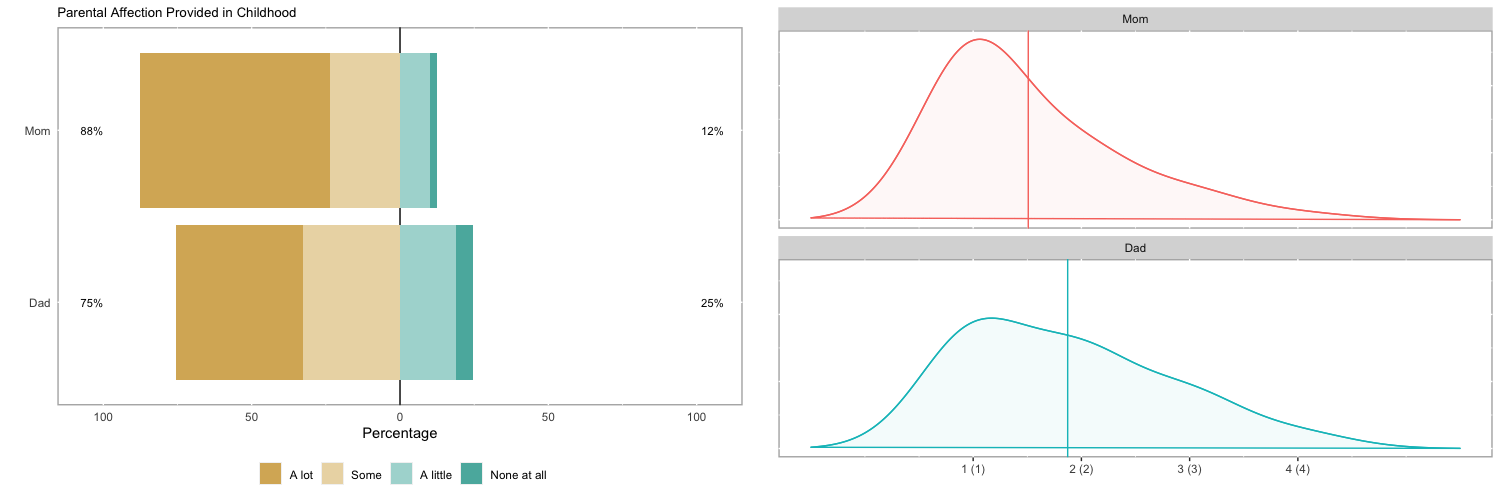
\includegraphics[scale=0.3]{likert1.png}
\end{figure}	

\begin{center}
\singlespacing
\textbf{Figure 1.} Distribution of responses regarding maternal and paternal affection in childhood in the 2014 CRCS.
\end{center}

In analyzing the relation between parental affection in childhood reported by respondents and psychological distress of respondents in adulthood, we aggregated the four likert-scale categories of reported parental affection into two dichotomous categories; ``a lot" and ``some" were categorized as high parental affection, whereas ``a little" and ``none at all" were categorized as low parental affection. Figure 2 shows the distribution of the outcome variable (i.e., psychological distress adulthood) for respondents reporting low vs. high maternal affection in childhood, as well as low vs. high paternal affection in childhood. 

\begin{figure}[H]
	\centering
	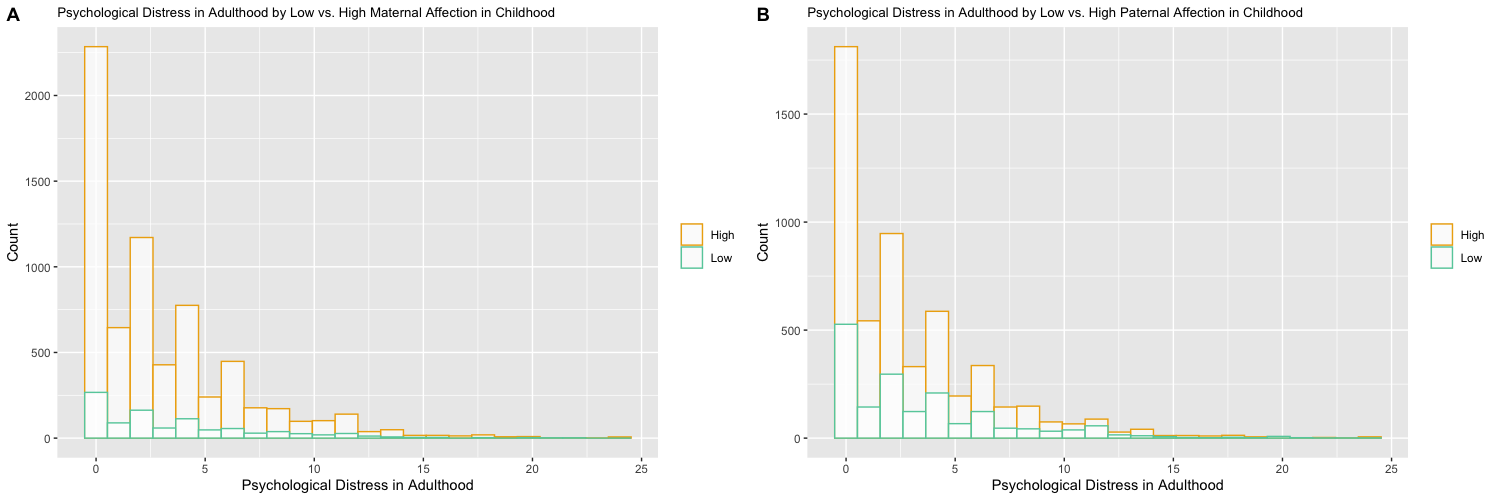
\includegraphics[scale=0.32]{histogram1.png}
\end{figure}	

\begin{center}
	\singlespacing
	\textbf{Figure 2.} Distribution of the outcome variable (psychological distress in adulthood) for respondents reporting (a) low vs. high maternal affection in childhood, and (b) low vs. high paternal affection in childhood. 
\end{center}

We performed multivariate linear regression to assess whether maternal or paternal affection in childhood as reported by respondents would be significant predictors of the respondent's psychological distress in adulthood. Maternal affection in childhood significantly predicted psychological distress in adulthood, b=.30, \textit{t}(7069) =2.16, \textit{p} = .03. Paternal affection in childhood also significantly predicted psychological distress in adulthood, b=.25, \textit{t}(7069) =2.41, \textit{p} = .02.  There was no reliable interaction between maternal and paternal affection in childhood on predicting psychological distress in adulthood. Full results of the regression analysis can be viewed in Appendix A. 

We also checked the normality, linearity, and constant variance assumptions of regression by creating the four diagnostic plots included in Figure 3. The residuals vs. fitted plot showed that the residuals are non-random, showing that there is systematic change in the spread of residuals over the range of fitted values (i.e., nonconstant variance) and that they are not centered around zero. The residuals were also distributed relatively randomly around the residual = 0 line, suggesting that the assumption that the relationship is linear is reasonable. This was consistent with the trends shown in the scale-location plot, as the studentized residuals = 0 line is approximately horizontal. As also shown by the density plot in Figure 1, the Q-Q plot reflected a right-skewed distribution. In assessing leverage, studentized residuals, and Cook's distance with the bubble plot, a few outliers were detected. However, we did not exclude outliers from our analysis. Results of the outlier test are included in Appendix A. 

\begin{figure}[H]
	\centering
	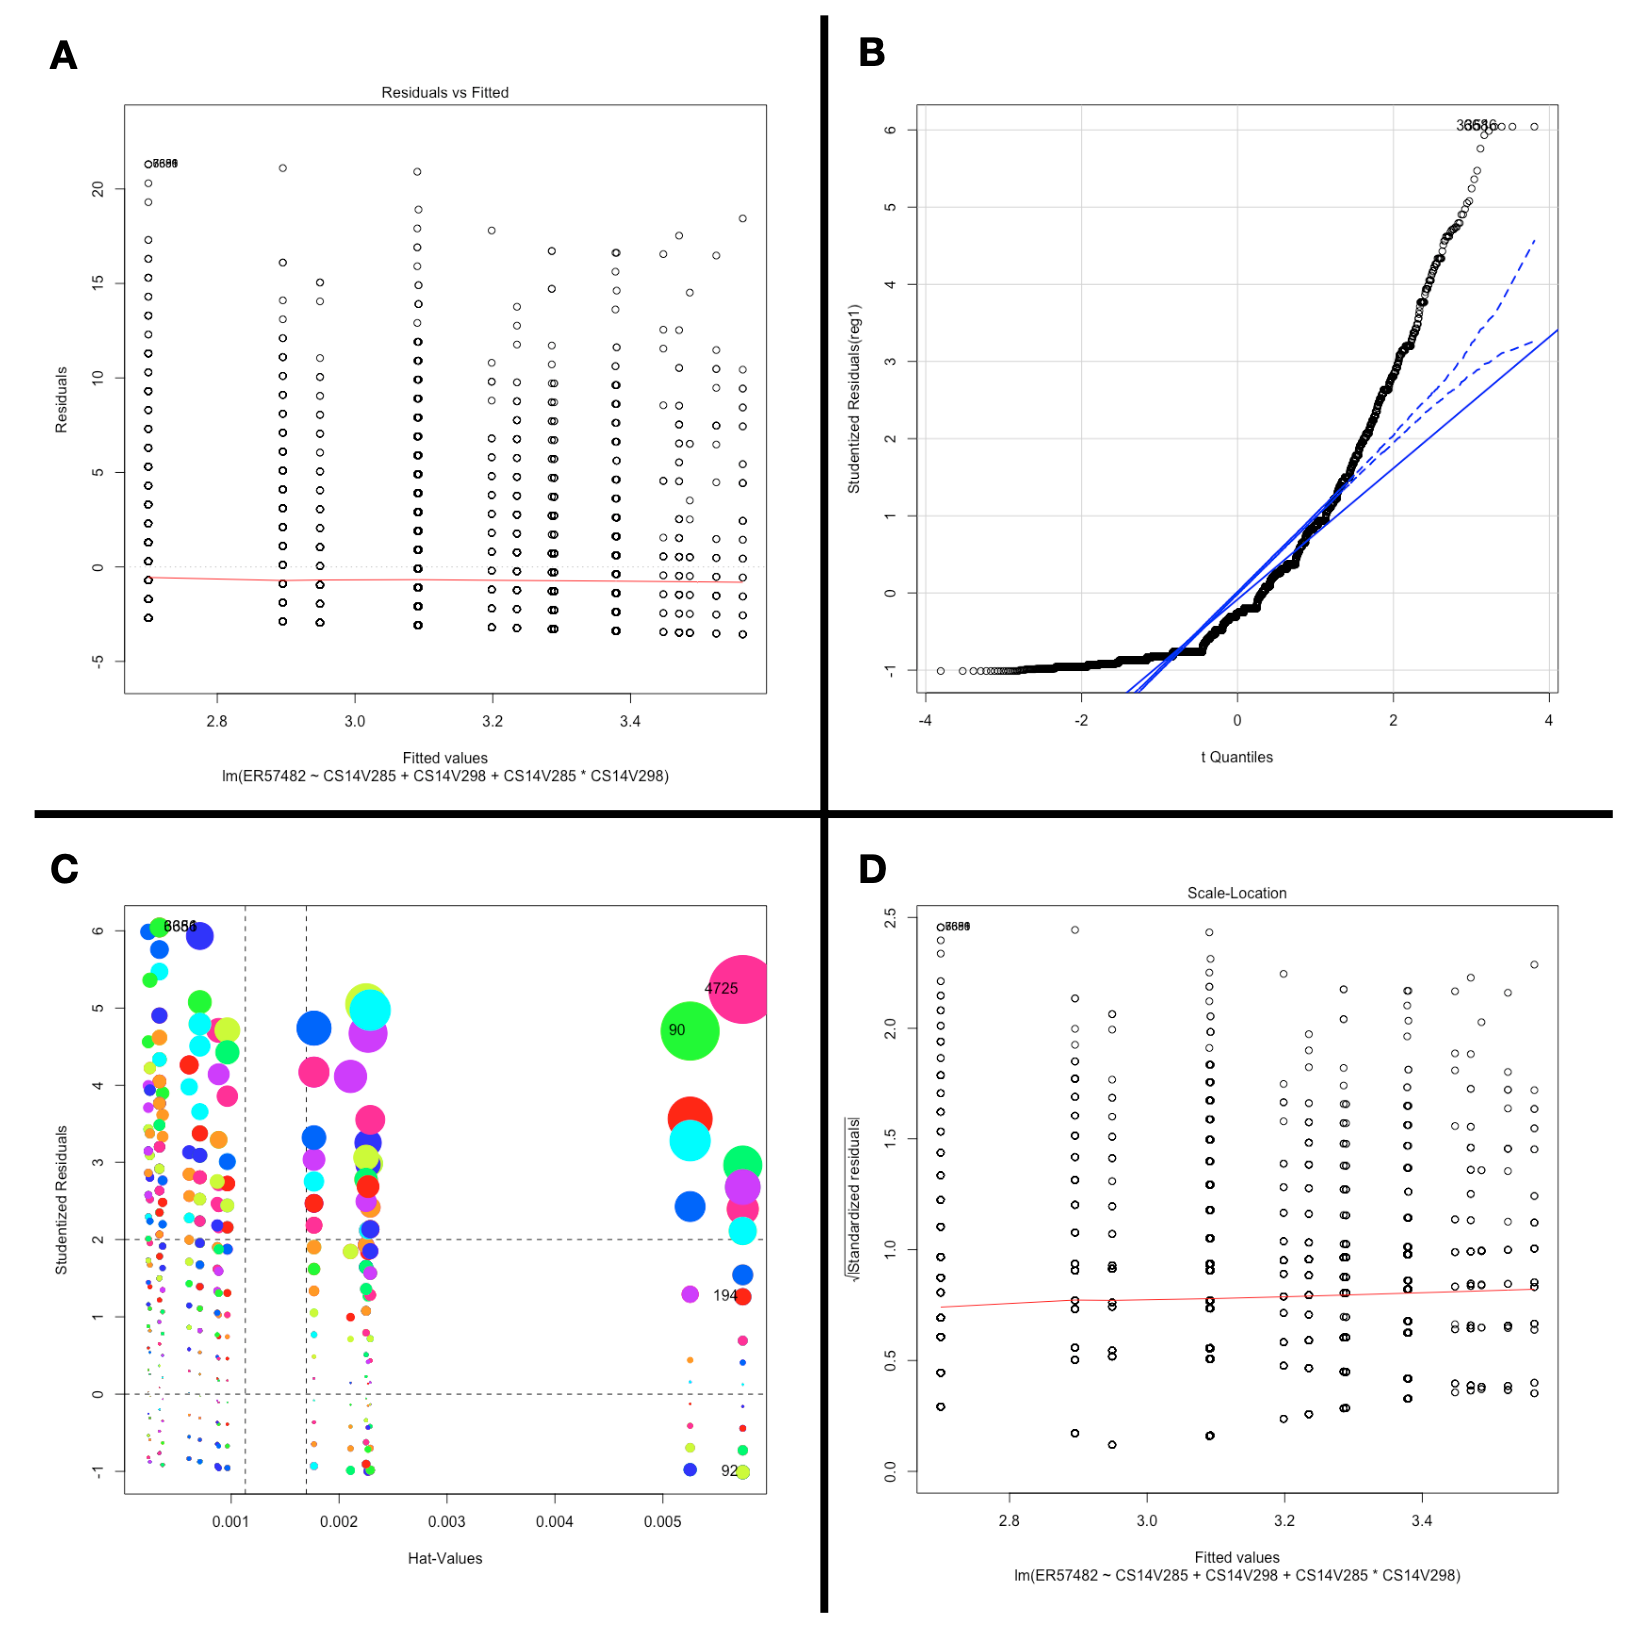
\includegraphics[scale=0.4]{reg1_asps.png}
\end{figure}	

\begin{center}
	\singlespacing
	\textbf{Figure 3.} Diagnostic plots for regression assessing  maternal and paternal affection in childhood as predictors of psychological distress in adulthood: (a) residuals vs. fitted plot, (b) normal Q-Q plot, (c) bubble plot, (d) scale-location plot.
\end{center}

\noindent{\textbf{II. Effect of parental strictness in childhood on psychological distress in adulthood}}

In the second section of this study, we hypothesized that the respondent's retrospective measure of parental strictness in childhood (maternal and paternal) would be significant predictors of the respondent's psychological distress in adulthood. Figure 4 shows the distribution of responses fom the 2014 CRCS survey regarding parental strictness in childhood, measured on a likert scale of 1 (\textit {Very}) to 4 (\textit{Not at all}). \\
\indent Approximately 34.47\% of respondents reported having had a very strict mom,  45.01\% reported having had a somewhat strict mom, 16.09\% reported having had a somewhat strict mom, and 4.43\% reported having had a mom who was not strict at all. Approximately 38.89\% of respondents reported having had a very strict dad,  38.7\% reported having had a somewhat strict dad, 15.8\% reported having had a not very strict dad, and 6.61\% reported having had a dad who was not strict at all. The level of maternal strictness in childhood reported by respondents (\textit{M}=1.9, \textit{SD}=0.82) was not significantly different from the level of paternal strictness in childhood reported by respondents (\textit{M} = 1.9, \textit{SD} = 0.9), \textit{t}(14500) = 0.25, \textit{p} =0.81.

\begin{figure}[H]
	\centering
	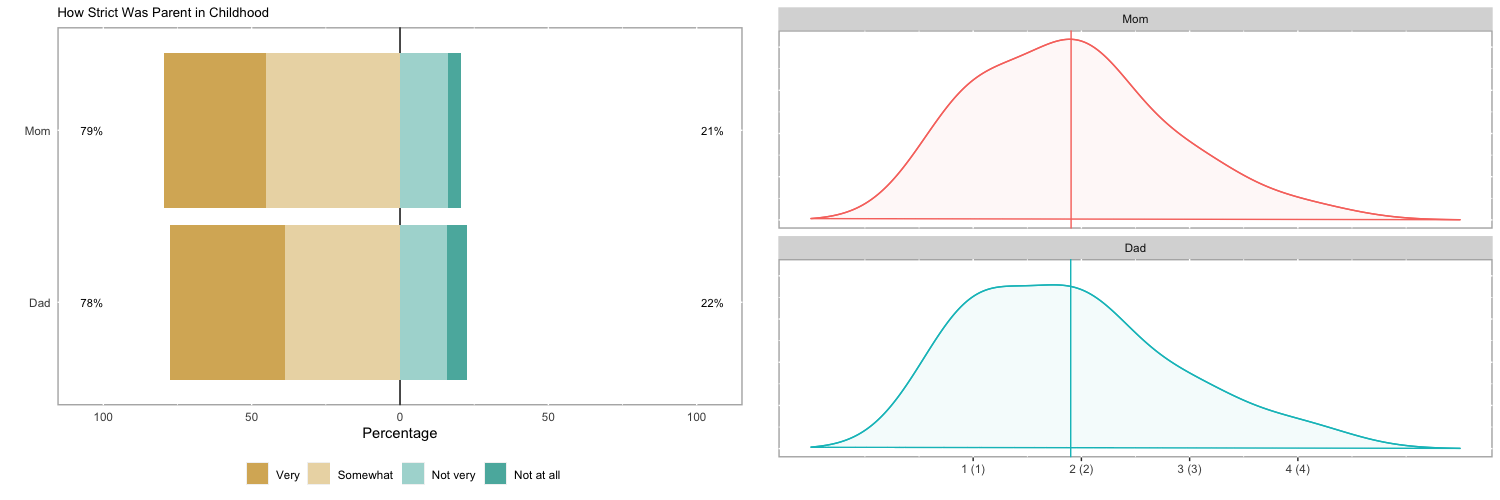
\includegraphics[scale=0.3]{likert2.png}
\end{figure}	
\begin{center}
	\singlespacing
	\textbf{Figure 4.} Distribution of responses regarding maternal and paternal strictness in childhood in the 2014 CRCS.
\end{center}

In analyzing the relation between parental strictness in childhood reported by respondents and psychological distress of respondents in adulthood, we again aggregated the four likert-scale categories of reported parental strictness into two dichotomous categories; ``very" and ``somewhat" were categorized as high parental strictness, whereas ``not very" and ``not at all" were categorized as low parental strictness. Figure 5 shows the distribution of the outcome variable (i.e., psychological distress adulthood) for respondents reporting low vs. high maternal strictness in childhood, as well as low vs. high paternal strictness in childhood. 

\begin{figure}[H]
	\centering
	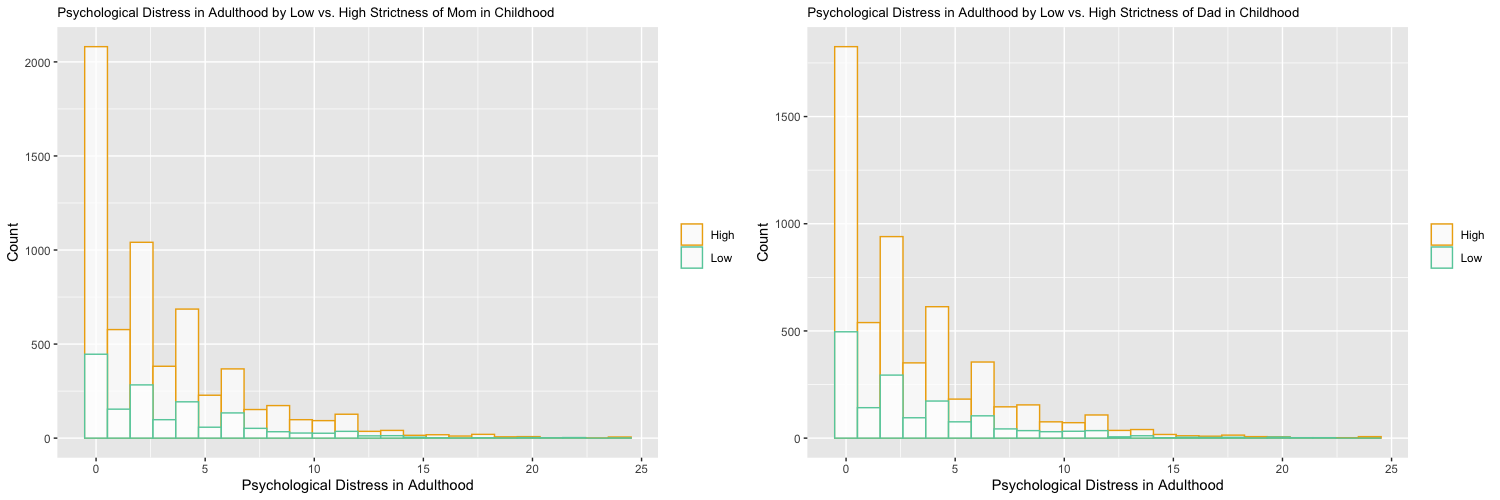
\includegraphics[scale=0.32]{histogram2.png}
\end{figure}	

\begin{center}
	\singlespacing
	\textbf{Figure 5.} Distribution of the outcome variable (psychological distress in adulthood) for respondents reporting (a) low vs. high maternal strictness in childhood, and (b) low vs. high paternal strictness in childhood. 
\end{center}

We performed multivariate linear regression to assess whether maternal or paternal strictness in childhood as reported by respondents would be significant predictors of the respondent's psychological distress in adulthood. Neither maternal nor paternal strictness in childhood significantly predicted psychological distress in adulthood. There was also no reliable interaction between maternal and paternal strictness in childhood on predicting psychological distress in adulthood. Full results of the regression analysis can be viewed in Appendix B. 

We also checked the normality, linearity, and constant variance assumptions of regression by creating the four diagnostic plots included in Figure 6.  The residuals vs. fitted plot and scale-location confirmed the constant variance assumption. As also shown by the density plot in Figure 4, the Q-Q plot reflected a slightly right-skewed distribution. A few outliers were detected by the bubble plot. However, we did not exclude outliers from our analysis. Results of the outlier test are included in Appendix B. 

\begin{figure}[H]
	\centering
	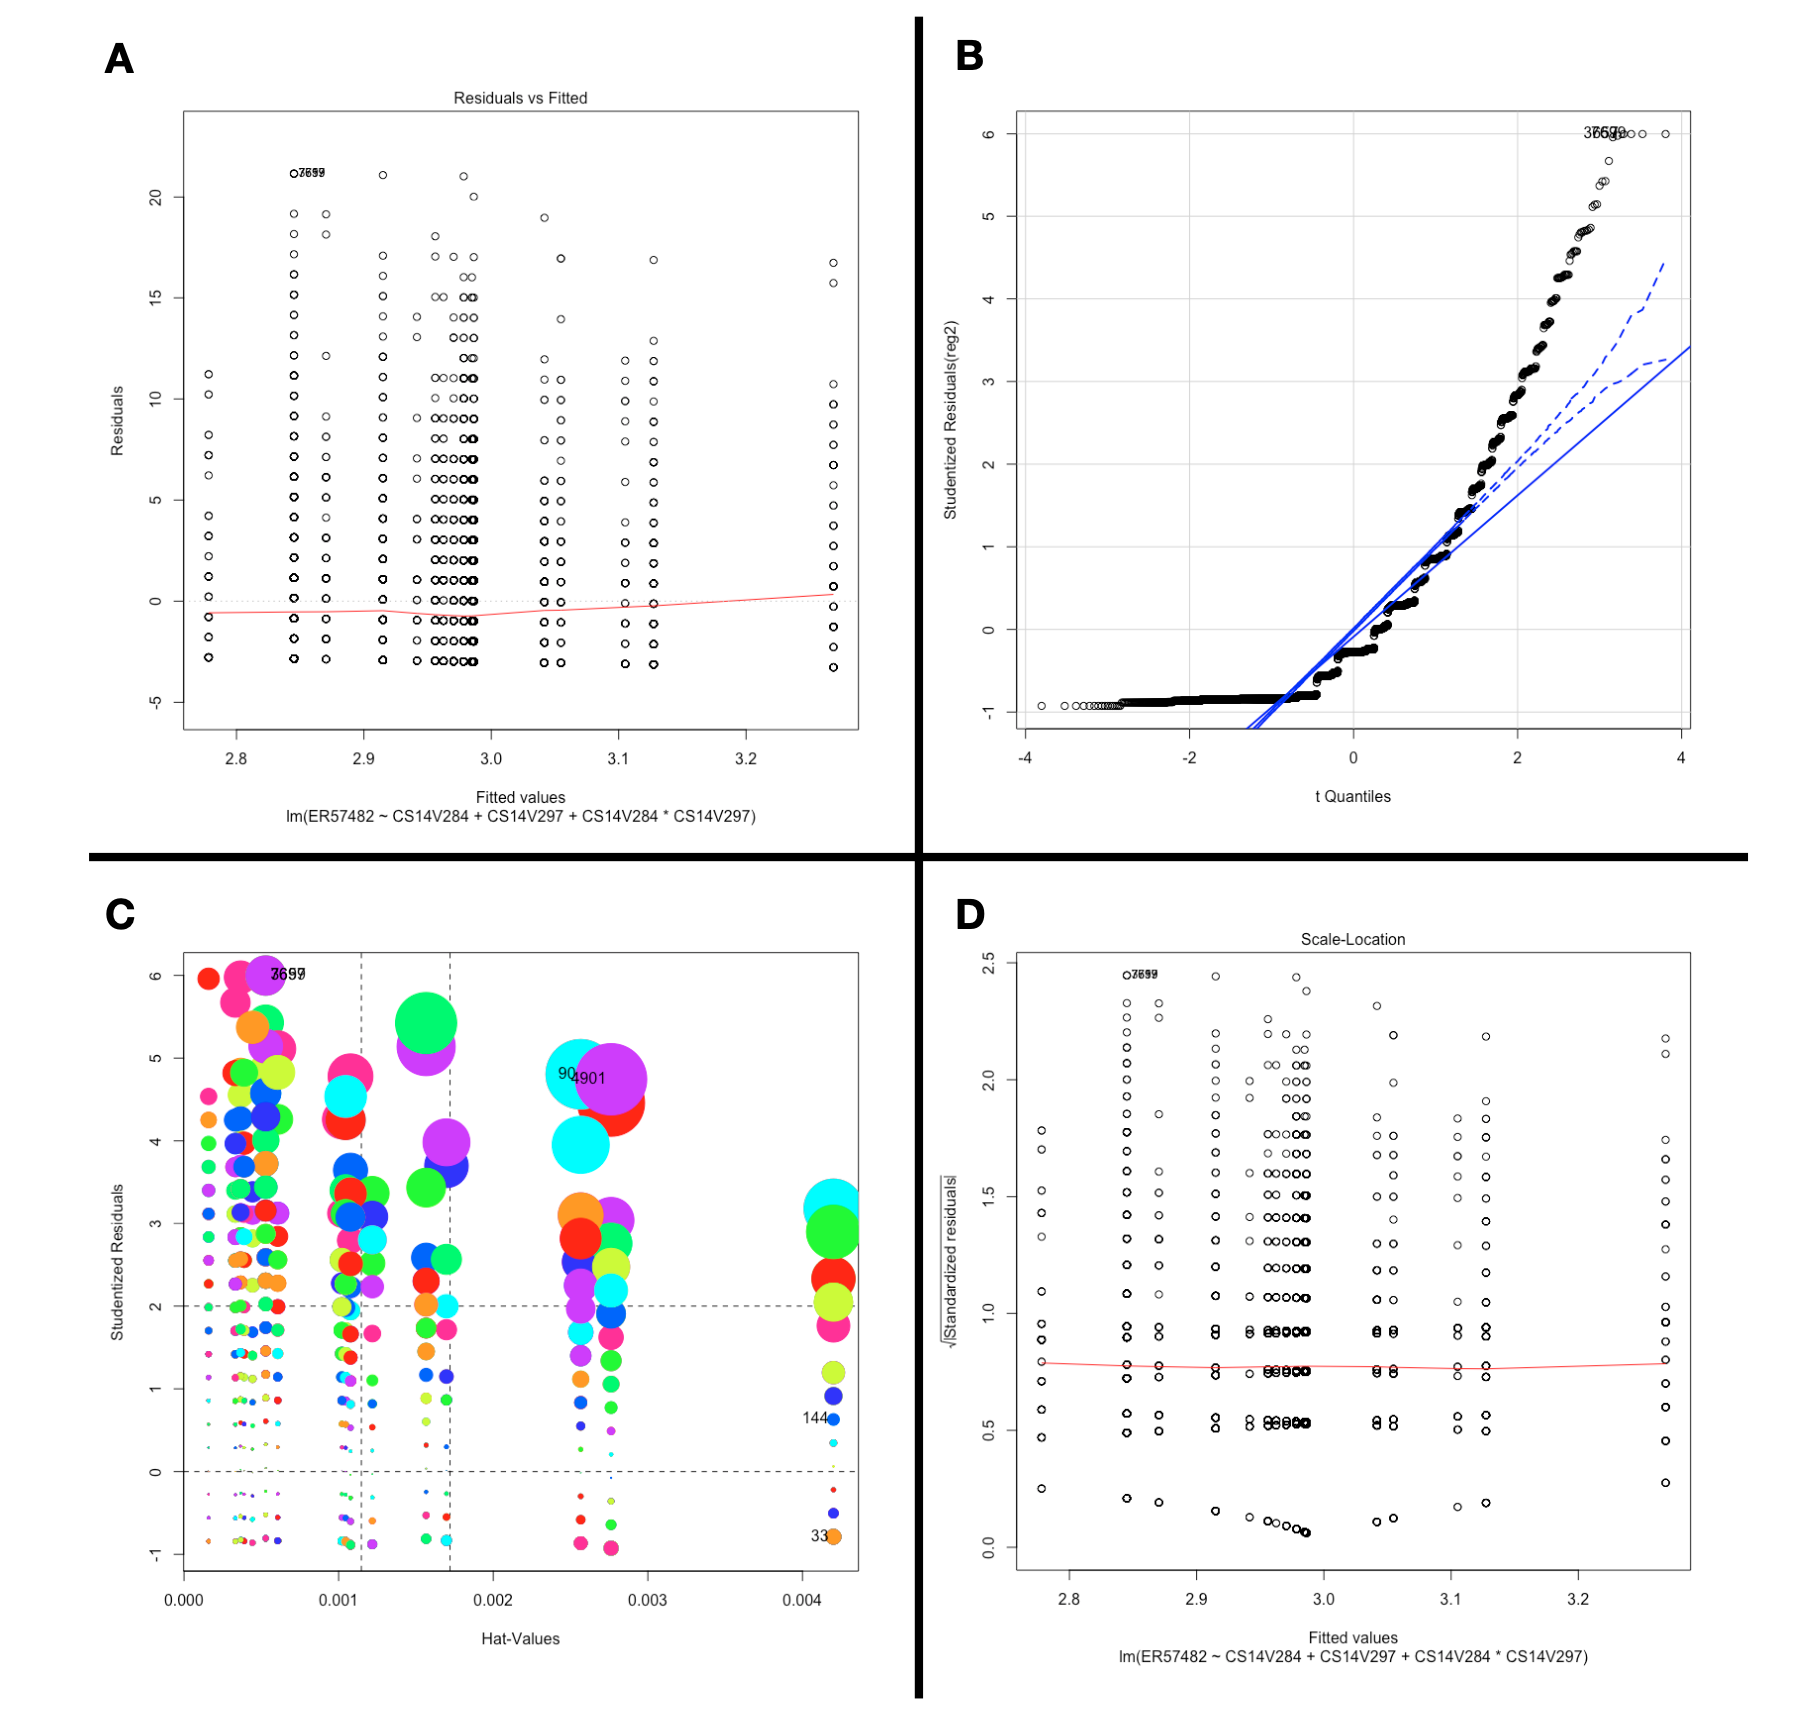
\includegraphics[scale=0.4]{reg2_asps.png}
\end{figure}	

\begin{center}
	\singlespacing
	\textbf{Figure 6.} Diagnostic plots for regression assessing maternal and paternal strictness in childhood as predictors of psychological distress in adulthood: (a) residuals vs. fitted plot, (b) normal Q-Q plot, (c) bubble plot, (d) scale-location plot.
\end{center}

\noindent{\textbf{III. Effect of relationship quality with parent in childhood on psychological distress in adulthood}}

In the third section of this study, we hypothesized that the respondent's retrospective measure of relationship quality with parents (mom and dad) would be significant predictors of the respondent's psychological distress in adulthood. Figure 4 shows the distribution of responses fom the 2014 CRCS survey regarding relationship quality with parents in childhood, measured on a likert scale of 1 (\textit {Excellent}) to 5 (\textit{Poor}). \\
\indent Approximately 36.88\% of respondents reported having had an excellent relationship with mom,  28.51\% reported having had a very good relationship with mom, 20.8\% reported having had a good relationship with mom, 10.36\% reported having had a fair relationship with mom, and 3.45\% reported having had poor relationship with mom. Approximately 25.69\% of respondents reported having had an excellent relationship with dad,  28.2\% reported having had a very good relationship with dad, 25.83\% reported having had a good relationship with dad, 13.72\% reported having had a fair relationship with dad, and 6.55\% reported having had poor relationship with dad. The level of relationship quality with mom in childhood as reported by respondents (\textit{M}=2.15, \textit{SD}=1.13) was significantly different from the level of relationship quality with dad in childhood as reported by respondents (\textit{M} = 2.47, \textit{SD} = 1.20), \textit{t}(14720) = -16.95, \textit{p} $<.01$.

\begin{figure}[H]
	\centering
	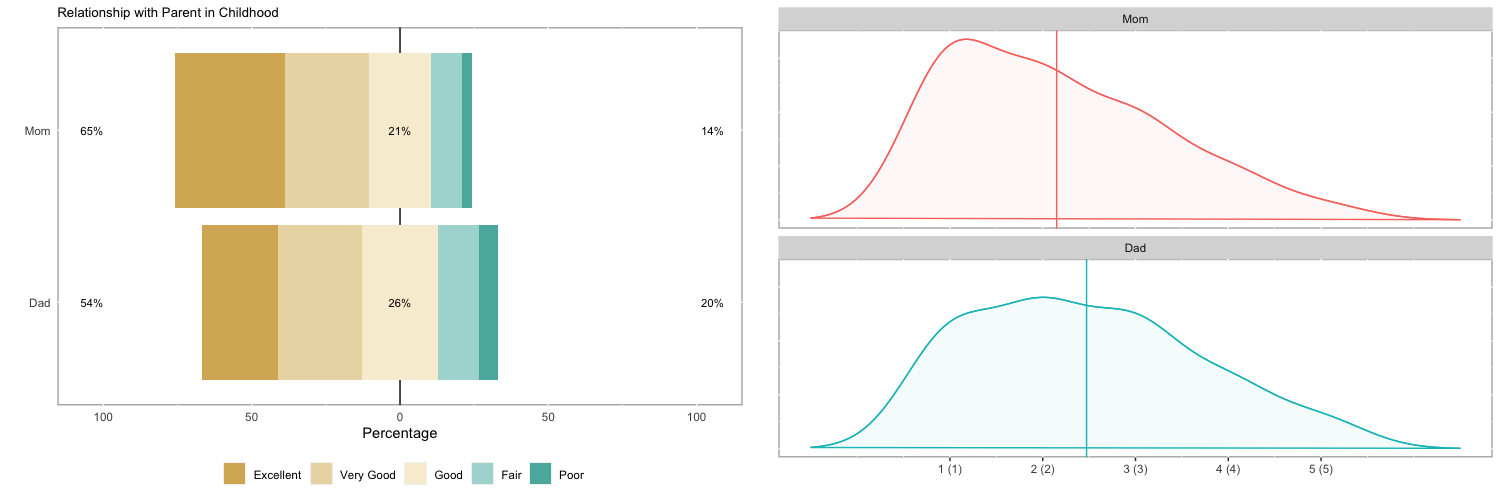
\includegraphics[scale=0.3]{likert3.png}
\end{figure}	

\begin{center}
	\singlespacing
	\textbf{Figure 7.} Distribution of responses regarding relationship quality with parents in childhood in the 2014 CRCS.
\end{center}

In analyzing the relations between relationship quality with parents in childhood as reported by respondents and psychological distress of respondents in adulthood, we aggregated the five likert-scale categories of quality of relationship with parents in childhood into two dichotomous categories; ``excellent", ``very good", and ``good" were categorized as high relationship quality, whereas ``fair" and ``poor" were categorized as low relationship quality. Figure 8 shows the distribution of the outcome variable (i.e., psychological distress adulthood) for respondents reporting low vs. high relationship quality with mom in childhood, as well as low vs. high relationship quality with dad in childhood. 

\begin{figure}[H]
	\centering
	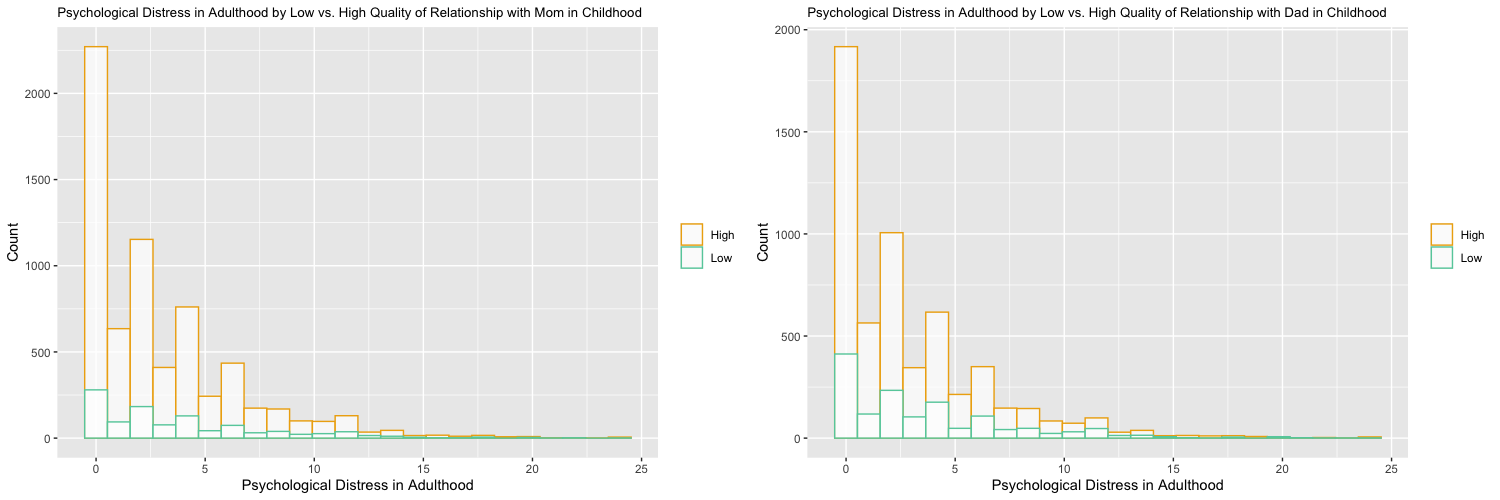
\includegraphics[scale=0.32]{histogram3.png}
\end{figure}	

\begin{center}
	\singlespacing
	\textbf{Figure 8.} Distribution of the outcome variable (psychological distress in adulthood) for respondents reporting (a) low vs. high relationship quality with mom in childhood, and (b) low vs. high relationship quality with dad in childhood. 
\end{center}

We performed multivariate linear regression to assess whether relationship quality with parents in childhood as reported by respondents would be significant predictors of the respondent's psychological distress in adulthood. Neither relationship quality with mom nor dad in childhood significantly predicted psychological distress in adulthood. There was also no reliable interaction between relationship quality with mom and relationship quality with dad in childhood on predicting psychological distress in adulthood. Full results of the regression analysis can be viewed in Appendix C. 

Normality, linearity, and constant variance assumptions of regression were again checked by creating the four diagnostic plots included in Figure 9.  The residuals vs. fitted  and scale-location plots showed that the constant variance assumption held. As also shown by the density plot in Figure 7, the Q-Q plot reflected a right-skewed distribution. Outliers were detected by the bubble plot. However, the outliers were not excluded. Results of the outlier test are included in Appendix C. 

\begin{figure}[H]
	\centering
	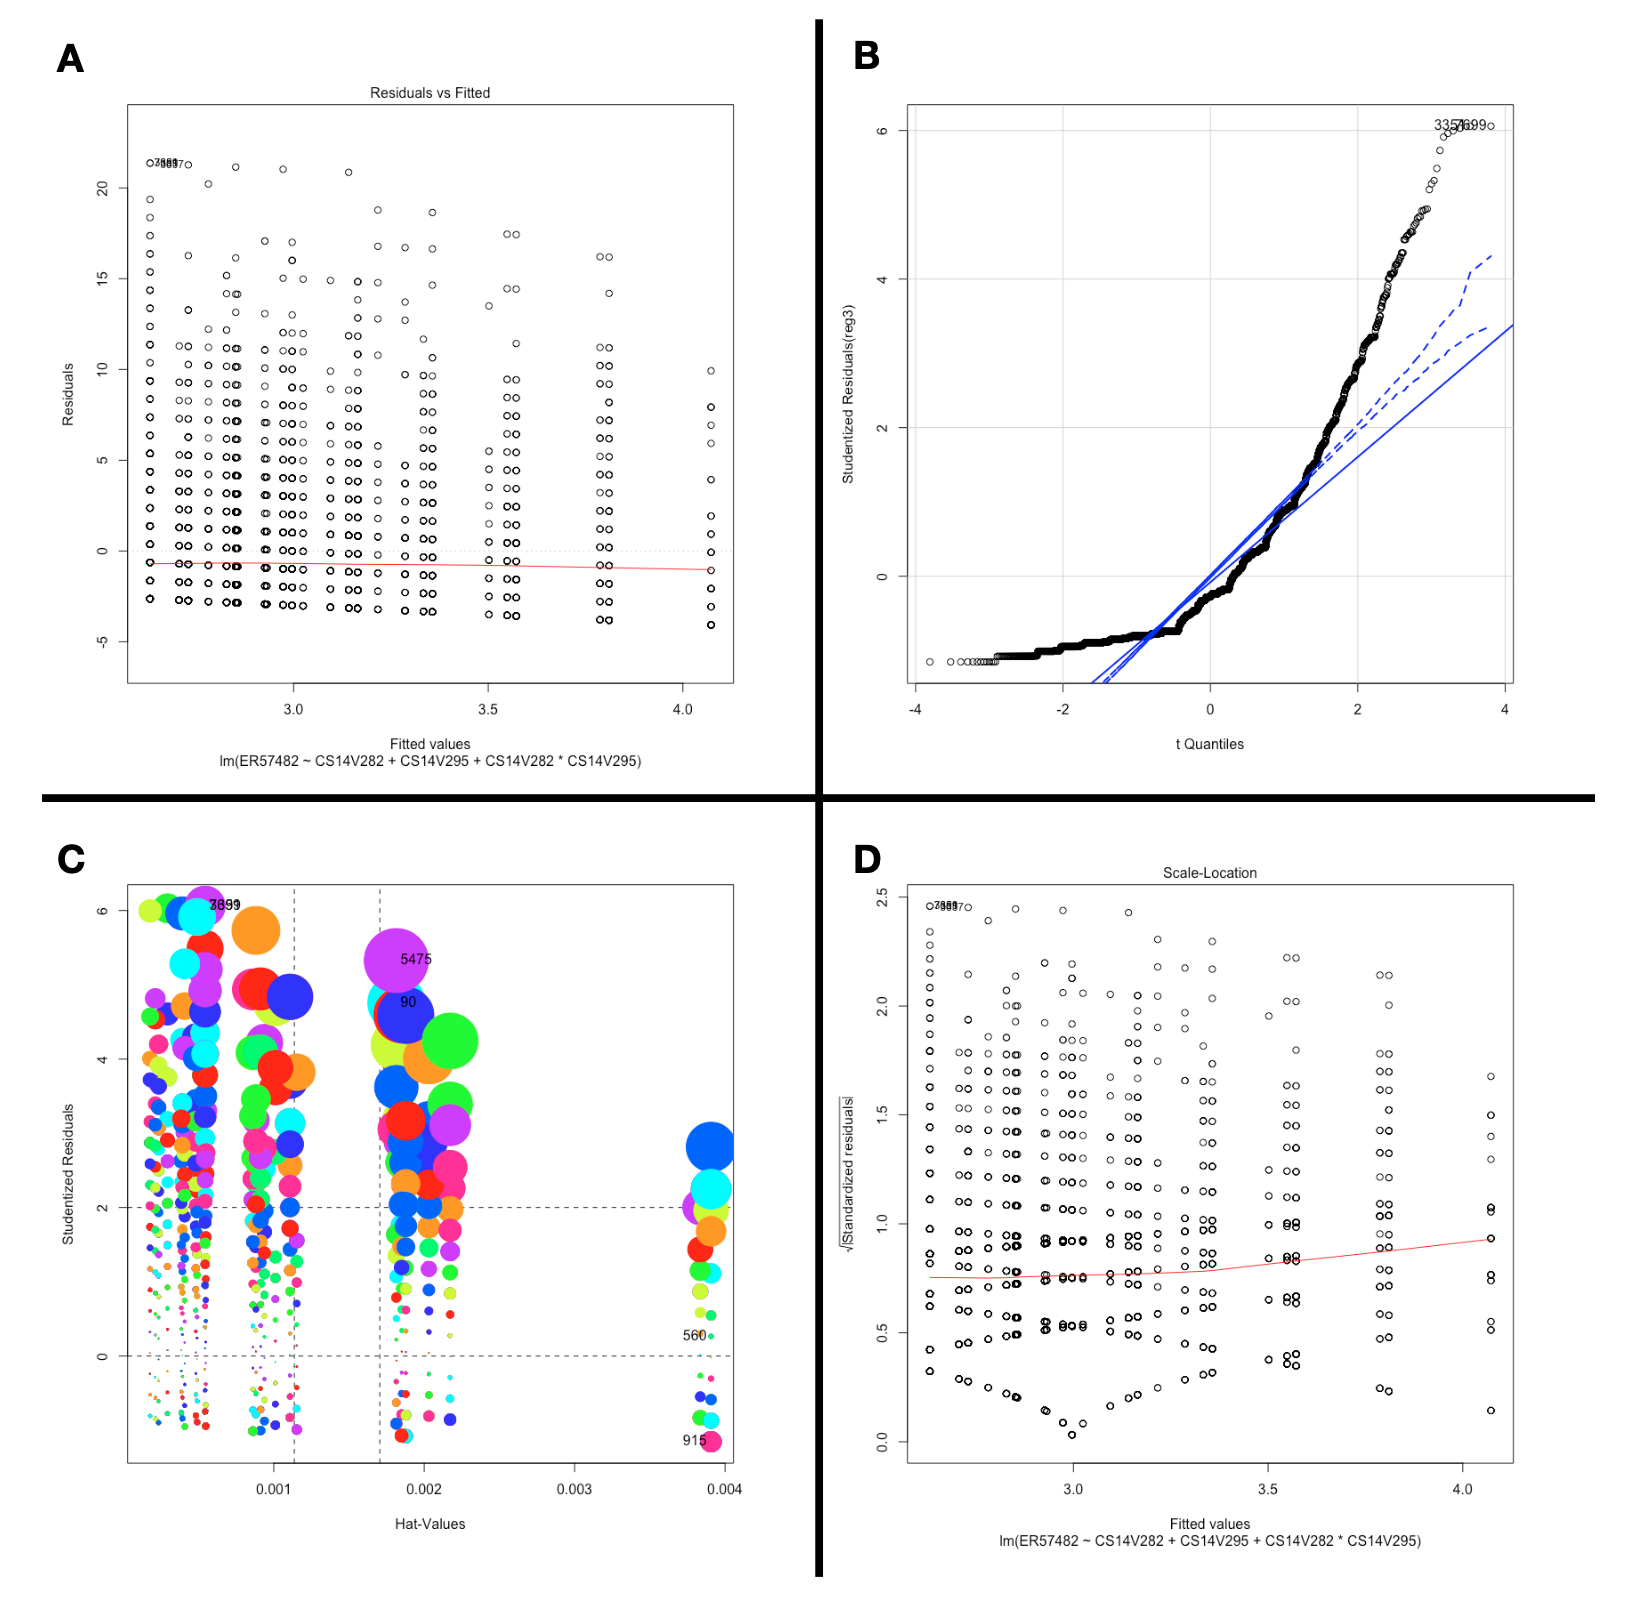
\includegraphics[scale=0.4]{reg3_asps.png}
\end{figure}

\begin{center}
	\singlespacing
	\textbf{Figure 9.} Diagnostic plots for regression assessing relationship quality with mom and dad in childhood as predictors of psychological distress in adulthood: (a) residuals vs. fitted plot, (b) normal Q-Q plot, (c) bubble plot, (d) scale-location plot.
\end{center}

\pagebreak
\begin{center}
	\noindent{\textbf{References}}
\end{center}

\noindent Aafjes-van Doorn, K., McCollum, J., Silberschatz, G., Kealy, D., \& Snyder, J. (2020).  \\
\indent Perceived adverse parenting in childhood and psychological distress among \\
\indent  psychotherapy patients. \textit{Journal of Nervous \& Mental Disease, 209}(3), 181–187. \\
\indent https://doi.org/10.1097/nmd.0000000000001274

\noindent Barnett, R. C., Kibria, N., Baruch, G. K., \& Pleck, J. H. (1991). Adult daughter- \\
\indent parent relationships and their associations with daughters' subjective \\
\indent well-being and psychological distress. \textit{Journal of Marriage and the Family,} \\ 
\indent \textit{53}(1), 29. https://doi.org/10.2307/353131

\noindent Baumrind, D., Larzelere, R. E., \& Owens, E. B. (2010). Effects of preschool parents' \\
\indent power assertive patterns and practices on Adolescent Development. \textit{Parenting,} \\
\indent \textit{10}(3), 157–201. https://doi.org/10.1080/15295190903290790

\noindent Chambers, J., Power, K., Loucks, N., \& Swanson, V. (2001). The interaction of \\ 
\indent perceived maternal and paternal parenting styles and their relation with the \\ 
\indent psychological distress and offending characteristics of incarcerated young \\ 
\indent offenders. \textit{Journal of Adolescence, 24}(2), 209–227. \\ 
\indent https://doi.org/10.1006/jado.2001.0377 

\noindent Davids, E. L., Roman, N. V., \& Leach, L. (2017). The link between parenting \\
\indent approaches and Health Behavior: A Systematic Review. \textit{Journal of Human} \\ 
\indent \textit{Behavior in the Social Environment, 27}(6), 589–608. \\ 
\indent https://doi.org/10.1080/10911359.2017.1311816 

\noindent Kessler, R. C., Barker, P. R., Colpe, L. J., Epstein, J. F., Gfroerer, J. C., Hiripi, E., \\ 
\indent Howes, M. J., Normand, S.-L. T., Manderscheid, R. W., Walters, E. E., \& \\ 
\indent Zaslavsky, A. M. (2003). Screening for serious mental illness in the general \\ 
\indent population. \textit{Archives of General Psychiatry, 60}(2), 184. \\ 
\indent https://doi.org/10.1001/archpsyc.60.2.184 

\noindent Khalid, J., \& Naeem, A. (2012). Relationships among life stress, perceived \\ 
\indent family environment, and the psychological distress of spina bifida adolescents. \\ 
\indent \textit{Family Issues in Pediatric Psychology, 43}(2), 55–76. \\
\indent https://doi.org/10.4324/9780203763063-7 

\noindent Morris, A. S., Criss, M. M., Silk, J. S., \& Houltberg, B. J. (2017). The impact of \\
\indent parenting on emotion regulation during childhood and adolescence. \textit{Child}\\
\indent \textit{Development Perspectives, 11}(4), 233–238. https://doi.org/10.1111/cdep.12238 

\noindent Musick, K., \& Meier, A. (2012). Assessing causality and persistence in associations \\
\indent between Family Dinners and adolescent well-being. \textit{Journal of Marriage} \\ 
\indent \textit{and Family, 74}(3), 476–493. https://doi.org/10.1111/j.1741-3737.2012.00973.x

\noindent Staples, L. G., Dear, B. F., Gandy, M., Fogliati, V., Fogliati, R., Karin, E., \\
\indent Nielssen, O., \& Titov, N. (2019). Psychometric Properties and clinical utility \\ 
\indent of brief measures of depression, anxiety, and general distress: The PHQ-2, \\ 
\indent Gad-2, and K-6. \textit{General Hospital Psychiatry, 56}, 13–18. \\ 
\indent https://doi.org/10.1016/j.genhosppsych.2018.11.003 


\pagebreak
\begin{center}
	\noindent{\textbf{Appendix A}}
\end{center}

\lstinputlisting[language=R, firstline=76, lastline=95]{EdaAnalysis.R}  
\pagebreak 

\VerbatimInput[fontsize=\small]{reg1.txt}
\pagebreak

\lstinputlisting[language=R, firstline=115, lastline=117]{EdaAnalysis.R}  
\VerbatimInput[fontsize=\small]{outliertest1.txt}

\begin{center}
	\noindent{\textbf{Appendix B}}
\end{center}

\lstinputlisting[language=R, firstline=207, lastline=226]{EdaAnalysis.R}  

\VerbatimInput[fontsize=\small]{reg2.txt}

\lstinputlisting[language=R, firstline=243, lastline=245]{EdaAnalysis.R}  
\VerbatimInput[fontsize=\small]{outliertest2.txt}

\begin{center}
	\noindent{\textbf{Appendix C}}
\end{center}

\lstinputlisting[language=R, firstline=340, lastline=359]{EdaAnalysis.R}  

\VerbatimInput[fontsize=\small]{reg3.txt}

\lstinputlisting[language=R, firstline=375, lastline=377]{EdaAnalysis.R}  
\VerbatimInput[fontsize=\small]{outliertest3.txt}

\begin{center}
	\noindent{\textbf{Appendix D}}
\end{center}

The work was divided evenly between authors. All authors contributed in background, dataset research, and coding. The abstract and introduction sections were completed by Michelle Bardales. The method section was completed by Yasmine Guedira. The summary statistics, data description, and measures of central tendency section was completed by Caroline Lee.  

\pagebreak
\let\clearpage\relax

\end{document}